\chapter{The Island of Tiboulen}

Dantès, although stunned and almost suffocated, had sufficient presence
of mind to hold his breath, and as his right hand (prepared as he was
for every chance) held his knife open, he rapidly ripped up the sack,
extricated his arm, and then his body; but in spite of all his efforts
to free himself from the shot, he felt it dragging him down still
lower. He then bent his body, and by a desperate effort severed the
cord that bound his legs, at the moment when it seemed as if he were
actually strangled. With a mighty leap he rose to the surface of the
sea, while the shot dragged down to the depths the sack that had so
nearly become his shroud.

Dantès waited only to get breath, and then dived, in order to avoid
being seen. When he arose a second time, he was fifty paces from where
he had first sunk. He saw overhead a black and tempestuous sky, across
which the wind was driving clouds that occasionally suffered a
twinkling star to appear; before him was the vast expanse of waters,
sombre and terrible, whose waves foamed and roared as if before the
approach of a storm. Behind him, blacker than the sea, blacker than the
sky, rose phantom-like the vast stone structure, whose projecting crags
seemed like arms extended to seize their prey, and on the highest rock
was a torch lighting two figures.

He fancied that these two forms were looking at the sea; doubtless
these strange grave-diggers had heard his cry. Dantès dived again, and
remained a long time beneath the water. This was an easy feat to him,
for he usually attracted a crowd of spectators in the bay before the
lighthouse at Marseilles when he swam there, and was unanimously
declared to be the best swimmer in the port. When he came up again the
light had disappeared.

He must now get his bearings. Ratonneau and Pomègue are the nearest
islands of all those that surround the Château d’If, but Ratonneau and
Pomègue are inhabited, as is also the islet of Daume. Tiboulen and
Lemaire were therefore the safest for Dantès’ venture. The islands of
Tiboulen and Lemaire are a league from the Château d’If; Dantès,
nevertheless, determined to make for them. But how could he find his
way in the darkness of the night?

At this moment he saw the light of Planier, gleaming in front of him
like a star. By leaving this light on the right, he kept the Island of
Tiboulen a little on the left; by turning to the left, therefore, he
would find it. But, as we have said, it was at least a league from the
Château d’If to this island. Often in prison Faria had said to him,
when he saw him idle and inactive:

“Dantès, you must not give way to this listlessness; you will be
drowned if you seek to escape, and your strength has not been properly
exercised and prepared for exertion.”

These words rang in Dantès’ ears, even beneath the waves; he hastened
to cleave his way through them to see if he had not lost his strength.
He found with pleasure that his captivity had taken away nothing of his
power, and that he was still master of that element on whose bosom he
had so often sported as a boy.

Fear, that relentless pursuer, clogged Dantès’ efforts. He listened for
any sound that might be audible, and every time that he rose to the top
of a wave he scanned the horizon, and strove to penetrate the darkness.
He fancied that every wave behind him was a pursuing boat, and he
redoubled his exertions, increasing rapidly his distance from the
château, but exhausting his strength. He swam on still, and already the
terrible château had disappeared in the darkness. He could not see it,
but he \textit{felt} its presence.

An hour passed, during which Dantès, excited by the feeling of freedom,
continued to cleave the waves.

“Let us see,” said he, “I have swum above an hour, but as the wind is
against me, that has retarded my speed; however, if I am not mistaken,
I must be close to Tiboulen. But what if I were mistaken?”

A shudder passed over him. He sought to tread water, in order to rest
himself; but the sea was too violent, and he felt that he could not
make use of this means of recuperation.

“Well,” said he, “I will swim on until I am worn out, or the cramp
seizes me, and then I shall sink;” and he struck out with the energy of
despair.

Suddenly the sky seemed to him to become still darker and more dense,
and heavy clouds seemed to sweep down towards him; at the same time he
felt a sharp pain in his knee. He fancied for a moment that he had been
shot, and listened for the report; but he heard nothing. Then he put
out his hand, and encountered an obstacle and with another stroke knew
that he had gained the shore.

Before him rose a grotesque mass of rocks, that resembled nothing so
much as a vast fire petrified at the moment of its most fervent
combustion. It was the Island of Tiboulen. Dantès rose, advanced a few
steps, and, with a fervent prayer of gratitude, stretched himself on
the granite, which seemed to him softer than down. Then, in spite of
the wind and rain, he fell into the deep, sweet sleep of utter
exhaustion. At the expiration of an hour Edmond was awakened by the
roar of thunder. The tempest was let loose and beating the atmosphere
with its mighty wings; from time to time a flash of lightning stretched
across the heavens like a fiery serpent, lighting up the clouds that
rolled on in vast chaotic waves.

Dantès had not been deceived—he had reached the first of the two
islands, which was, in fact, Tiboulen. He knew that it was barren and
without shelter; but when the sea became more calm, he resolved to
plunge into its waves again, and swim to Lemaire, equally arid, but
larger, and consequently better adapted for concealment.

An overhanging rock offered him a temporary shelter, and scarcely had
he availed himself of it when the tempest burst forth in all its fury.
Edmond felt the trembling of the rock beneath which he lay; the waves,
dashing themselves against it, wetted him with their spray. He was
safely sheltered, and yet he felt dizzy in the midst of the warring of
the elements and the dazzling brightness of the lightning. It seemed to
him that the island trembled to its base, and that it would, like a
vessel at anchor, break moorings, and bear him off into the centre of
the storm.

He then recollected that he had not eaten or drunk for four-and-twenty
hours. He extended his hands, and drank greedily of the rainwater that
had lodged in a hollow of the rock.

As he rose, a flash of lightning, that seemed to rive the remotest
heights of heaven, illumined the darkness. By its light, between the
Island of Lemaire and Cape Croiselle, a quarter of a league distant,
Dantès saw a fishing-boat driven rapidly like a spectre before the
power of winds and waves. A second after, he saw it again, approaching
with frightful rapidity. Dantès cried at the top of his voice to warn
them of their danger, but they saw it themselves. Another flash showed
him four men clinging to the shattered mast and the rigging, while a
fifth clung to the broken rudder. The men he beheld saw him
undoubtedly, for their cries were carried to his ears by the wind.
Above the splintered mast a sail rent to tatters was waving; suddenly
the ropes that still held it gave way, and it disappeared in the
darkness of the night like a vast sea-bird.

At the same moment a violent crash was heard, and cries of distress.
Dantès from his rocky perch saw the shattered vessel, and among the
fragments the floating forms of the hapless sailors. Then all was dark
again.

Dantès ran down the rocks at the risk of being himself dashed to
pieces; he listened, he groped about, but he heard and saw nothing—the
cries had ceased, and the tempest continued to rage. By degrees the
wind abated, vast gray clouds rolled towards the west, and the blue
firmament appeared studded with bright stars. Soon a red streak became
visible in the horizon, the waves whitened, a light played over them,
and gilded their foaming crests with gold. It was day.

Dantès stood mute and motionless before this majestic spectacle, as if
he now beheld it for the first time; and indeed since his captivity in
the Château d’If he had forgotten that such scenes were ever to be
witnessed. He turned towards the fortress, and looked at both sea and
land. The gloomy building rose from the bosom of the ocean with
imposing majesty and seemed to dominate the scene. It was about five
o’clock. The sea continued to get calmer.

“In two or three hours,” thought Dantès, “the turnkey will enter my
chamber, find the body of my poor friend, recognize it, seek for me in
vain, and give the alarm. Then the tunnel will be discovered; the men
who cast me into the sea and who must have heard the cry I uttered,
will be questioned. Then boats filled with armed soldiers will pursue
the wretched fugitive. The cannon will warn everyone to refuse shelter
to a man wandering about naked and famished. The police of Marseilles
will be on the alert by land, whilst the governor pursues me by sea. I
am cold, I am hungry. I have lost even the knife that saved me. Oh, my
God, I have suffered enough surely! Have pity on me, and do for me what
I am unable to do for myself.”

As Dantès (his eyes turned in the direction of the Château d’If)
uttered this prayer, he saw off the farther point of the Island of
Pomègue a small vessel with lateen sail skimming the sea like a gull in
search of prey; and with his sailor’s eye he knew it to be a Genoese
tartan. She was coming out of Marseilles harbor, and was standing out
to sea rapidly, her sharp prow cleaving through the waves.

“Oh,” cried Edmond, “to think that in half an hour I could join her,
did I not fear being questioned, detected, and conveyed back to
Marseilles! What can I do? What story can I invent? under pretext of
trading along the coast, these men, who are in reality smugglers, will
prefer selling me to doing a good action. I must wait. But I cannot—I
am starving. In a few hours my strength will be utterly exhausted;
besides, perhaps I have not been missed at the fortress. I can pass as
one of the sailors wrecked last night. My story will be accepted, for
there is no one left to contradict me.”

As he spoke, Dantès looked toward the spot where the fishing-vessel had
been wrecked, and started. The red cap of one of the sailors hung to a
point of the rock and some timbers that had formed part of the vessel’s
keel, floated at the foot of the crag. In an instant Dantès’ plan was
formed. He swam to the cap, placed it on his head, seized one of the
timbers, and struck out so as to cut across the course the vessel was
taking.

“I am saved!” murmured he. And this conviction restored his strength.

He soon saw that the vessel, with the wind dead ahead, was tacking
between the Château d’If and the tower of Planier. For an instant he
feared lest, instead of keeping in shore, she should stand out to sea;
but he soon saw that she would pass, like most vessels bound for Italy,
between the islands of Jaros and Calaseraigne.

However, the vessel and the swimmer insensibly neared one another, and
in one of its tacks the tartan bore down within a quarter of a mile of
him. He rose on the waves, making signs of distress; but no one on
board saw him, and the vessel stood on another tack. Dantès would have
shouted, but he knew that the wind would drown his voice.

It was then he rejoiced at his precaution in taking the timber, for
without it he would have been unable, perhaps, to reach the
vessel—certainly to return to shore, should he be unsuccessful in
attracting attention.

Dantès, though almost sure as to what course the vessel would take, had
yet watched it anxiously until it tacked and stood towards him. Then he
advanced; but before they could meet, the vessel again changed her
course. By a violent effort he rose half out of the water, waving his
cap, and uttering a loud shout peculiar to sailors. This time he was
both seen and heard, and the tartan instantly steered towards him. At
the same time, he saw they were about to lower the boat.

An instant after, the boat, rowed by two men, advanced rapidly towards
him. Dantès let go of the timber, which he now thought to be useless,
and swam vigorously to meet them. But he had reckoned too much upon his
strength, and then he realized how serviceable the timber had been to
him. His arms became stiff, his legs lost their flexibility, and he was
almost breathless.

He shouted again. The two sailors redoubled their efforts, and one of
them cried in Italian, “Courage!”

The word reached his ear as a wave which he no longer had the strength
to surmount passed over his head. He rose again to the surface,
struggled with the last desperate effort of a drowning man, uttered a
third cry, and felt himself sinking, as if the fatal cannon shot were
again tied to his feet. The water passed over his head, and the sky
turned gray. A convulsive movement again brought him to the surface. He
felt himself seized by the hair, then he saw and heard nothing. He had
fainted.

When he opened his eyes Dantès found himself on the deck of the tartan.
His first care was to see what course they were taking. They were
rapidly leaving the Château d’If behind. Dantès was so exhausted that
the exclamation of joy he uttered was mistaken for a sigh.

As we have said, he was lying on the deck. A sailor was rubbing his
limbs with a woollen cloth; another, whom he recognized as the one who
had cried out “Courage!” held a gourd full of rum to his mouth; while
the third, an old sailor, at once the pilot and captain, looked on with
that egotistical pity men feel for a misfortune that they have escaped
yesterday, and which may overtake them tomorrow.

A few drops of the rum restored suspended animation, while the friction
of his limbs restored their elasticity.

“Who are you?” said the pilot in bad French.

“I am,” replied Dantès, in bad Italian, “a Maltese sailor. We were
coming from Syracuse laden with grain. The storm of last night overtook
us at Cape Morgiou, and we were wrecked on these rocks.”

“Where do you come from?”

“From these rocks that I had the good luck to cling to while our
captain and the rest of the crew were all lost. I saw your vessel, and
fearful of being left to perish on the desolate island, I swam off on a
piece of wreckage to try and intercept your course. You have saved my
life, and I thank you,” continued Dantès. “I was lost when one of your
sailors caught hold of my hair.”

“It was I,” said a sailor of a frank and manly appearance; “and it was
time, for you were sinking.”

“Yes,” returned Dantès, holding out his hand, “I thank you again.”

“I almost hesitated, though,” replied the sailor; “you looked more like
a brigand than an honest man, with your beard six inches, and your hair
a foot long.”

Dantès recollected that his hair and beard had not been cut all the
time he was at the Château d’If.

“Yes,” said he, “I made a vow, to our Lady of the Grotto not to cut my
hair or beard for ten years if I were saved in a moment of danger; but
today the vow expires.”

“Now what are we to do with you?” said the captain.

“Alas, anything you please. My captain is dead; I have barely escaped;
but I am a good sailor. Leave me at the first port you make; I shall be
sure to find employment.”

“Do you know the Mediterranean?”

“I have sailed over it since my childhood.”

“You know the best harbors?”

“There are few ports that I could not enter or leave with a bandage
over my eyes.”

“I say, captain,” said the sailor who had cried “Courage!” to Dantès,
“if what he says is true, what hinders his staying with us?”

“If he says true,” said the captain doubtingly. “But in his present
condition he will promise anything, and take his chance of keeping it
afterwards.”

“I will do more than I promise,” said Dantès.

“We shall see,” returned the other, smiling.

“Where are you going?” asked Dantès.

“To Leghorn.”

“Then why, instead of tacking so frequently, do you not sail nearer the
wind?”

“Because we should run straight on to the Island of Rion.”

“You shall pass it by twenty fathoms.”

“Take the helm, and let us see what you know.”

The young man took the helm, felt to see if the vessel answered the
rudder promptly and seeing that, without being a first-rate sailor, she
yet was tolerably obedient.

“To the sheets,” said he. The four seamen, who composed the crew,
obeyed, while the pilot looked on. “Haul taut.”

They obeyed.

“Belay.” This order was also executed; and the vessel passed, as Dantès
had predicted, twenty fathoms to windward.

“Bravo!” said the captain.

“Bravo!” repeated the sailors. And they all looked with astonishment at
this man whose eye now disclosed an intelligence and his body a vigor
they had not thought him capable of showing.

“You see,” said Dantès, quitting the helm, “I shall be of some use to
you, at least during the voyage. If you do not want me at Leghorn, you
can leave me there, and I will pay you out of the first wages I get,
for my food and the clothes you lend me.”

“Ah,” said the captain, “we can agree very well, if you are
reasonable.”

“Give me what you give the others, and it will be all right,” returned
Dantès.

“That’s not fair,” said the seaman who had saved Dantès; “for you know
more than we do.”

“What is that to you, Jacopo?” returned the Captain. “Everyone is free
to ask what he pleases.”

“That’s true,” replied Jacopo; “I only make a remark.”

“Well, you would do much better to find him a jacket and a pair of
trousers, if you have them.”

“No,” said Jacopo; “but I have a shirt and a pair of trousers.”

“That is all I want,” interrupted Dantès. Jacopo dived into the hold
and soon returned with what Edmond wanted.

“Now, then, do you wish for anything else?” said the patron.

“A piece of bread and another glass of the capital rum I tasted, for I
have not eaten or drunk for a long time.” He had not tasted food for
forty hours. A piece of bread was brought, and Jacopo offered him the
gourd.

“Larboard your helm,” cried the captain to the steersman. Dantès
glanced that way as he lifted the gourd to his mouth; then paused with
hand in mid-air.

“Hollo! what’s the matter at the Château d’If?” said the captain.

A small white cloud, which had attracted Dantès’ attention, crowned the
summit of the bastion of the Château d’If. At the same moment the faint
report of a gun was heard. The sailors looked at one another.

“What is this?” asked the captain.

“A prisoner has escaped from the Château d’If, and they are firing the
alarm gun,” replied Dantès. The captain glanced at him, but he had
lifted the rum to his lips and was drinking it with so much composure,
that suspicions, if the captain had any, died away.

\begin{figure}[ht]
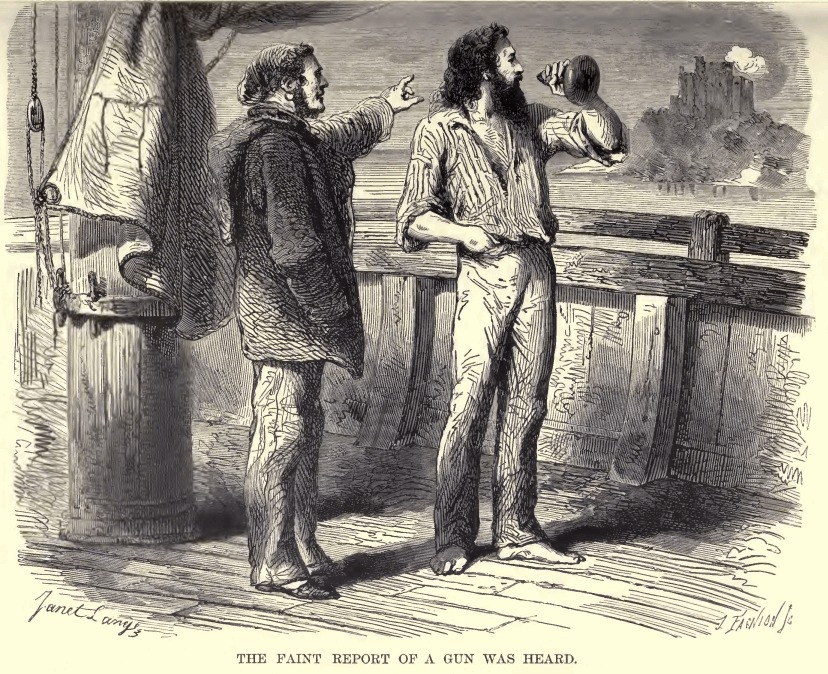
\includegraphics[width=\textwidth]{0277m.jpg}
\end{figure}

“Pretty strong rum!” said Dantès, wiping his brow with his sleeve.

“At any rate,” murmured he, “if it be, so much the better, for I have
made a rare acquisition.”

\begin{figure}[ht]
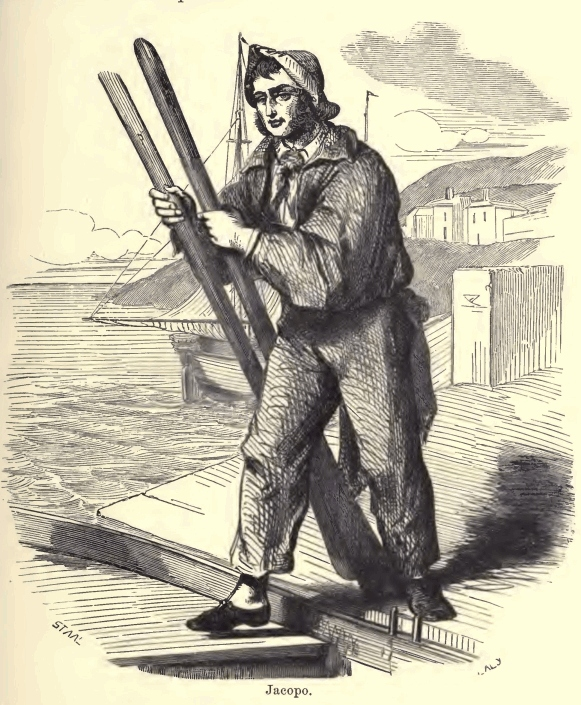
\includegraphics[width=\textwidth]{0279m.jpg}
\end{figure}

Under pretence of being fatigued, Dantès asked to take the helm; the
steersman, glad to be relieved, looked at the captain, and the latter
by a sign indicated that he might abandon it to his new comrade. Dantès
could thus keep his eyes on Marseilles.

“What is the day of the month?” asked he of Jacopo, who sat down beside
him.

“The 28th of February.”

“In what year?”

“In what year—you ask me in what year?”

“Yes,” replied the young man, “I ask you in what year!”

“You have forgotten then?”

“I got such a fright last night,” replied Dantès, smiling, “that I have
almost lost my memory. I ask you what year is it?”

“The year 1829,” returned Jacopo.

It was fourteen years, day for day, since Dantès’ arrest. He was
nineteen when he entered the Château d’If; he was thirty-three when he
escaped. A sorrowful smile passed over his face; he asked himself what
had become of Mercédès, who must believe him dead. Then his eyes
lighted up with hatred as he thought of the three men who had caused
him so long and wretched a captivity. He renewed against Danglars,
Fernand, and Villefort the oath of implacable vengeance he had made in
his dungeon.

This oath was no longer a vain menace; for the fastest sailor in the
Mediterranean would have been unable to overtake the little tartan,
that with every stitch of canvas set was flying before the wind to
Leghorn.
